\chapter{Velocity reconstruction using regression} 
\label{chap_linearregression} 

This chapter presents regression models to address the problem of estimating high resolution fields from low resolution measurements as defined in section \ref{sec:probdef1}. It reviews the basic ordinary least squares model, regularized linear regression with the common L2 penalty as well as the L1 penalty, and kernel regression. These models are presented in matrix forms, which are more compact than previous works on turbulence. The problem of selecting model complexity and optimizing model parameters, a fundamental topic in learning theory, are also discussed. 

The models are used to reconstruct high-resolution fields from low-resolution measurements. The DNS database of isotropic turbulence presented in section \ref{sec:data_isotropic} are used for illustration. Only partial results on selecting the models and optimizing parameters are shown in this chapter. Optimal models will be used in chapter \ref{chap_comparisons} when comparing performances of all proposed models. 

\section{Regression in turbulence studies}
Regression is probably the earliest method in statistics for prediction. It aims at learning the relation between input variables and corresponding output targets. The model is learned from training samples where both input and output variables are available. the learned model will be used for prediction in situations where only input variables are given. Nice reviews can be found in \citet{bishop2006pattern} and \citet{hastie2009elements}. 

Least squares regression has been applied widely in turbulence studies under the name ``\textit{linear stochastic estimation}'' (LSE) \citep{adrian1977role,adrian1979conditional}. It has been further investigated \citep{guezennec1989stochastic,adrian1992stochastic,ewing1999examination} to estimate conditional eddies from the measurements. Later works introduced various extensions such as multi-time, nonlinear or higher-order LSE \citep{mokhasi2009predictive,durgesh2010multi,nguyen2010proper,meyer2014provide}, which reconstruct velocity fields from pressure or shear-stress measurements. LSE can be also linked to proper orthogonal decomposition (POD), known also as ``principle component analysis'', to reduce the order of reconstruction problems \citep{bonnet1994stochastic}. 

The idea of combining LR velocity measurements to obtain HR fields using regression has not been addressed until recently \citep{melnick2012experimental,tu2013integration}. \citet{melnick2012experimental} used a POD-LSE model to get fully resolved 3D velocities of a flow over a flat plate by combining 3D smoke intensity and 2D PIV measurements. The POD-LSE model has been developed further by \citet{tu2013integration} with a multi-time LSE reconstruction model. Kalman filter or Kalman smoother are used as real time estimation or data post-processing respectively. The model is tested using time-resolved PIV measurements of a bluff-body wake at a low $ Re $.

Regression models in previous works remains rather simple, with the use of POD to reduce the order of the model. However, simple linear regression models suffer from certain limitations. The use of POD, acting as a low-pass filter, neglects certain small scales \textit{a priori}. This work discusses further extensions of simple linear regression based on different regularizations or kernel methods. We aim at maximizing the amount of information that each method can recover, so POD is left aside throughout the thesis. Detailed analysis of reconstruction results such as spectra and errors will assess the performances of regression models as mapping functions between large and small scales. 

\section{Ordinary least squares (OLS)}
Given a set of $ \dimtl $ training samples $ \left\lbrace \left(\y_t, \z_t\right)\right\rbrace, t= 1,2,...,\dimtl $ corresponding to pairs of inputs $ \y_t \in \R^{\dimsl}$ and outputs $ \z_t \in \R^{\dimsh}$, regression models estimate $ \z_t $ as a function of $\y_t $ via a mapping function $ f $: 
\begin{equation}
	f:  \y_t \mapsto  \myhat{\z }_t = f(\y_t) + \n_t
\end{equation}
where $ \n_t \sim \mathscr{N}(0,\sigma^2_{\n_t})$ is usually a white Gaussian noise. $ f $ is learned from the $ \dimtl $ pairs of training samples. This function should minimize the loss $ \loss(f) $, which measures how far the prediction $ f(\y) $ and the reference $ \z $ are different within the training data.

The ordinary least squares model (OLS) assumes that $ f $ is a empirical linear function of $ \y_t $. This model is widely used for its simplicity yet efficiency in situations where only a small training set with low signal-to-noise ratio is given. Assuming that $ \{\z_t\} $ and $ \{\y_t\} $ are mean-free and pre-normalized to one-standard deviation, OLS is expressed as:
\begin{equation}
\myhat{\z }_t = f(\y_t) = \B^{\mytrans}\y_t
\end{equation}
where  $ \B $ is the coefficient matrix of size $ \dimsl \times \dimsh $. The $ i- $th column of $ \B $ tells how to weight each measurement  $ \y_{t,j} $ to get an estimate of $ \z_{t,i} $. The unknown $ \B $ is learned from training data by minimizing the empirical loss:
\begin{equation}
\loss(\B) = \sum^{\dimtl}_{t=1}{ \normtwo{\z_t-\B^{\mytrans}\y_t}	}
\end{equation}
or rearranged in the matrix form as:
\begin{equation}
\loss(\B) = \normtwo{\Y\B-\Z} = \left(\Y\B-\Z\right)^{\mytrans}\left(\Y\B-\Z\right)
\label{eq:LSE2}
\end{equation}
where $ \Y^{\mytrans} \mydef \{\y_t\} $ of size $ \dimsl \times \dimtl $ and $ \Z^{\mytrans} \mydef \{\z_t \} $ of size $\dimsh \times \dimtl$. $ \normtwo{.} $ is the Euclidean distance, also called ``\textit{L2 norm}''. $ \mydef $ is the notation of ``\textit{define as}''. The loss $ \loss(\B) $ is the square of errors, which is purely data-dependent. The optimization problem is to finds $ \B $ such that:
\begin{equation}
\B= \argmin_B{ \left\lbrace \loss(\B) \right\rbrace} = \argmin_B{ \left\lbrace\Vert \Y\B-\Z\Vert^2_2 \right\rbrace}
\end{equation}
$ \argmin{ \{ . \}} $ is the argument of the minimum seeking $ \B $ such that $ \loss(\B) $ attains its minimum. The least square error solution of $ \B $ is by differentiating equation \ref{eq:LSE2} with respect to $\B$ and set to zero:
\begin{equation}
\B= \pinv { \Y } \Z= \left( \Y^{\mytrans}\Y \right)^{-1} \Y^{\mytrans}\Z
\label{eq:LSE5}
\end{equation}
where $ (.)\pinv{} $ is Moore-Penrose pseudo inverse. Then, the output $ \z^\ext  $ of any new input vector $ \y^\ext$ out of the training set is estimated as:
\begin{equation}
\z^\ext = \B^{\mytrans}\y^\ext
\label{eq:LSE6}
\end{equation} 

\section{Regularized linear regression}
\label{sec:regularized_linear_regression}
OLS suffers from critical problems. It requires the inverse of matrix $ \Y^{\mytrans}\Y $ that can be singular or almost singular. The iterative solver can overcome this problem, but may result in a high-variance model with many large coefficients: a small change of $\y^\ext$ leads to very different predictions of $\z^\ext$. Since learned purely from the training data, it often fits very well the training data but poorly performs otherwise. This phenomena is called \textit{overfitting} and will be discussed later in this chapter. Regularized least squares are proposed to overcome this problem. The idea is to add a regularization term $ g(\B) $ on $ \B $ to the data-dependent error term:
\begin{equation}
	\loss(\B, \lambda) = \Vert \Y\B-\Z\Vert^2_2 +\lambda g(\B)
	\label{eq:regularized_linear_regression1}
\end{equation}
where the regularization parameter $ \lambda $ controls the balance between the two terms. Different terms lead to different regression models.

\subsection{Ridge Regression (RR): L2 penalty}
\label{sec:l2_penalty}
The most common and simple regularization is L2 penalty, also called ``weight decay'', which leads to the formulation of ridge regression (RR). The regularization term is on the norm of OLS coefficients, i.e. $ g(\B) = \Vert \B \Vert^2_2$. The loss function becomes:
\begin{equation}
\loss(\B, \lambda) = \Vert \Y\B-\Z\Vert^2_2 +\lambda\Vert \B \Vert^2_2 
\label{eq:RR1}
\end{equation}
The parameter $\lambda $ controls the balance between the data misfit and regularization term, which is the sum of squares of all coefficients. It controls how far $ \B $ are shrunk towards zero, the larger $ \lambda $ the further. Setting the derivative with respect to $ \B $ to zero, the closed form to estimate $ \B $ is:
\begin{equation}
\B=\left( \Y ^{\mytrans}\Y+\lambda \I \right)^{-1}  \Y ^{\mytrans}\Z 
\label{eq:RR2}
\end{equation}
This formula is similar to that of OLS except that some positive value $ \lambda $ is added to the diagonal elements of $ \Y^{\mytrans}\Y $ to ensure $ \Y^{\mytrans}\Y +\lambda \I$ is always invertible.

The mechanism of RR can be analyzed via the singular value decomposition (SVD) of $ \Y $: 
\begin{equation}
\Y= \Umat\Diag\Vmat^{\mytrans}
\label{eq:RR3}
\end{equation}
where $ \Umat=(\mybold{u}_1, \mybold{u}_2,... ,\mybold{u}_{\dimsl}) $ is a $ \dimtl \times \dimsl $ orthogonal matrix, $ \Diag = diag(d_1, d_2, ... , d_{\dimsl} )$ is a $ \dimsl \times \dimsl $ diagonal matrix $ (d_1 \geq d_2 \geq ... \geq d_{\dimsl}) $, and $ \Vmat^{\mytrans}=(\mybold{v}_1^{\mytrans}, \mybold{v}_2^{\mytrans},... ,\mybold{v}_{\dimsl}^{\mytrans}) $ is a $ \dimsl \times \dimsl $ orthogonal matrix. The orthogonality implies that $ \Umat^{\mytrans}\Umat = \I $ or $ \Umat^{\mytrans}=\Umat^{-1} $, similarly for $ \Vmat $ and $ \Vmat^{\mytrans} $. The formula to estimate RR coefficients becomes:
\begin{equation}
\B =\left(\Y^{\mytrans} \Y + \lambda \I\right)^{-1}\Y^{\mytrans}\Z = \Vmat \, diag \left( \frac{d_j^2}{d_j^2+\lambda} \right) \, \Umat^{\mytrans} \Z
\label{eq:RR6}
\end{equation}
Re-estimating training output variables $ \Z $ as a function of inputs, one obtains:
\begin{equation}
\myhat{\Z} = \Y\B = \sum\limits_{j=1}^{\dimsl} \left( \mybold{u}_j \frac{d_j^2}{d_j^2 + \lambda} \mybold{u}^{\mytrans}\right)\Z
\label{eq:RR8}
\end{equation}
This implies that RR projects $ \Z $ onto the principal components of $ \Y^{\mytrans}\Y $ with large energy content (large $ d_j $) and shrinks the coefficients of low energy (small $ d_j $). This makes RR close to the \textit{principal component regression} model discussed in \citet{jolliffe1982note}, where one decomposes $ \Y^{\mytrans}\Y $ using SVD and then set components with low energy content (small $ d_j $) to zeros in a handy manner. The approach also avoids matrix inversion and plays a role similar to regularization.

\subsection{LASSO: L1 penalty}
\label{sec:l1_penalty}
The nature of L2 penalty  is to reduce model variance by shrinking coefficients corresponding to irrelevant events toward zero. However, they are not exactly zero. L1 penalty will precisely force some coefficients to zero. The model is called least absolute selection and shrinkage operator (LASSO) \citep{tibshirani1996regression} in statistics, or basis pursuit denoising (BPDN) \citep{chen1998atomic} in signal processing. It is considered as an implicit subset selection step, where irrelevant events are neglected from the reconstruction. This property favors sparsity - output is estimated as a combination of some input variables only- that is beneficial in many applications.

\begin{algorithm}[t]
\caption{Iterative shrinkage-thresholding algorithm (ISTA)}\label{algo_ISTA}
\begin{algorithmic}[1]
\State Set k=0 and initialize $ \B^{(0)} $; 
\While{not convergence}
	\State $ \bigtriangledown f(\B^{(k)}) = \Y^{\mytrans}(\Z-\Y\B^{(k)})$ \Comment{Residual from step k}
	\State $\B^{(k+1)} \gets \prox_{\lambda \normone{.}} \left[ \B^{(k)} - t^{(k)} \bigtriangledown f(\B^{(k)}) \right] $
	\State k = k + 1 
\EndWhile
\State \textbf{return} $\B^{(k+1)}$
\end{algorithmic}
\end{algorithm}
 
The LASSO cost function is similar to that of RR with a subtle but very important modification:
\begin{equation}
F(\B)= \Vert \Y\B-\Z\Vert^2_2 +\lambda \normone{\B}
\label{eq: LASSO1}
\end{equation}
The data-dependent term is the same as OLS or RR. The different penalty term $ \lambda \normone{\B}$ imposes a constraint on the sum of absolute values of coefficients. This modification leads to sparsity, the key difference between LASSO and RR. It also makes the problem nonlinear and there exits no closed-form solution. Gradient-based methods are usually used to solve this optimization problem. Iterative shrinkage-thresholding algorithms (ISTA) is one of them, where $ \B $ is solved iteratively by \textit{soft-thresholding} as in Algorithm \ref{algo_ISTA} \citep{daubechies2004iterative}. In the pseudo code, $ prox $- the shrinkage operator- is the element-wise soft-thresholding: 
\begin{equation}
\left(\prox_{\lambda \normone{.}}[\B]\right)_i =
\begin{cases}
b_i-\lambda \mysign{b_i} & \text{if } |b_i|>\lambda,
\\
0 & \text{otherwise }
\end{cases}
\end{equation}
where $ t^{(k)} $ is the gradient step size, $ b_i $ is the $ i- $th coefficient of $ \B $. The \textit{sign function} $ \mysign{b_i} $ is defined as:
\begin{equation}
 \mysign{b_i} =
\begin{cases}
-1 & \text{if } b_i<0,
\\
0 & \text{if } b_i=0,
\\
1  & \text{if } b_i>0.
\end{cases}
\end{equation}
Faster schemes have been proposed to accelerate the convergence time \citep{vonesch2008fast,beck2009fast}, but further discussions are outside the scope of this work.

LASSO often outperforms RR and subset selection methods for several reasons. Compared to RR, LASSO takes most of the advantages, including the stability of the solution and the shrinkage feature. These features give a low-variance model compared to subset selection method. Moreover, LASSO favors sparsity, which can be considered as an implicit subset selection \citep{hastie2005elements, hastie2009unsupervised}. By forcing some of the coefficients to zeros, the irrelevant predictors are suppressed in final estimation.

\section{Nonlinear regression}
\label{sec:nonlinear_regression}
Linear regression aims at mapping the output as a linear combination of input variables. This implies a real constraint on performances of this family of models. In many cases including turbulence, linear functions are too simple to describe the undergoing phenomenon. Nonlinear regression models are beneficial, and kernel feature mapping is often used.

\subsection{Feature mapping}
Kernel methods are used to introduce nonlinearity into the model. The idea is to project the original input vector $ \y  $ onto a fixed feature space:
\begin{equation}
\y_t \mymapto \mybold{\phi}_t = \featmap{\y_t}
\end{equation}
and perform least square regression in this space. $ \y_t \in \R^{\dimsl}$ is the $ t- $ input vector. The feature vector $ \mybold{\phi}_t \in \R^{\Df} $, where $ \Df \gg \dimsl $ is the dimension in feature space. The least square problem becomes: 
\begin{equation}
\B = \argmin_B{ \left\lbrace \normtwo{ \Z- \mathbf{\Phi}\B} \right\rbrace}
\end{equation}
where $ \mathbf{\Phi} = \{\mybold{\phi}_t \} $ ($ t = 1, ..., \dimtl $), the so-called \textit{design matrix}, is of size $ \dimtl \times \Df $. Adding L2 regularization term $ \normtwo{\B} $ and deriving analogously as RR model, the solution is:
\begin{equation}
\B=\left(\mathbf{\Phi}^{\mytrans}\mathbf{\Phi} + \lambda \I\right)^{-1}\mathbf{\Phi}^{\mytrans}\Z
\end{equation}
Then the prediction of a new input variable $ \y^\ext $ is:
\begin{equation}
\z^\ext=\B^{\mytrans} \featmap{\y^\ext}
\end{equation} 

\subsection{Kernel ridge regression}
Involving nonlinearity via feature mapping significantly increases computational costs. The kernel trick is proposed \citep{saunders1998ridge} to overcome this problem, resulting in the so-called kernel ridge regression (KRR) model. This trick appears when solving ridge regression using Lagrange dual optimization.

\subsubsection*{Dual form of ridge regression}
RR in equation \ref{eq:RR1} can be re-expressed as a dual Lagrangian optimization problem:
\begin{equation}
\B=\argmin_B{ \left\lbrace \sum\limits_{t=1}^{\dimtl}\normtwo{\mybold{e}_t} + \lambda \normtwo{\B} \right\rbrace } \subjectto \z_t - \B^{\mytrans}\y_t = \mybold{e}_t, \:\:\:\:\:\: t = 1, 2, ..., \dimtl
\label{eq:RRdual1}
\end{equation}
where $ s.t $ stands for ``\textit{subject to}''. Introducing Lagrange multipliers $ A[\dimtl \times \dimsh] \mydef \{\mybold{a}_t^{\mytrans} \} (t = 1, 2, ..., \dimtl), \mybold{a}_t \in \R^{\dimsh}$, the optimization problem \ref{eq:RRdual1} is equivalent to the problem of finding the saddle point of the function:
\begin{equation}
\sum\limits_{t=1}^{\dimtl}\normtwo{\mybold{e}_t} + \lambda \normtwo{\B} + \sum\limits_{t=1}^{\dimtl} \mybold{a}_t^{\mytrans}\left( \z_t - \B^{\mytrans}\y_t - \mybold{e}_t\right)
\end{equation}
The solution as shown in \citet{saunders1998ridge} is:
\begin{equation}
\mathbf{A}  = \left(\mathbf{K} + \lambda \I\right)^{-1}\Z
\end{equation}
where $ \mathbf{K} \mydef \Y\Y^{\mytrans} $ is the matrix of dot products, $ \mathbf{K}_{m,n} = \y _m^{\mytrans} \y _n $. The prediction for a new input variables $ \y^\ext $ is:
\begin{equation}
\myhat{\z }^\ext = \left(\sum\limits_{t=1}^{\dimtl}\mybold{a}_t^{\mytrans}\y_t\right)\y^\ext = \mathbf{A}^{\mytrans} \mybold{k}^{\ext}
\end{equation}
where $ \mybold{k}^{\ext} \mydef \{k_t\} = \{ \y_t^{\mytrans} \y^\ext \} \in \R^{\dimtl}$.
 
\subsubsection*{Kernel trick}

\begin{table}
\centering
\begin{tabular}{lc} \toprule
	Function name  & $ k (\mybold{u}, \mybold{v}) $ \\ \midrule
	Linear  & $ \mybold{u}^{\mytrans} \mybold{v} $ \\ \midrule
	Polynomial  & $ (r + \mybold{u}^{\mytrans} \mybold{v})^d $ for $ r,d \geq 0 $\\ \midrule
	Radial basis function (RBF)  & $ \myexp{-\gamma \normtwo{\mybold{u} - \mybold{v}}}$, $ \gamma > 0 $ \\
	\bottomrule
\end{tabular}
\caption{Common basis functions for kernel methods.}
\label{tab_basisfunctions}
\end{table}

Solving RR in the dual form offers no improvement of accuracy, speed or stability. However, the beauty of this approach is the presence of only dot products among input variables in the final prediction step. This implies an analogous procedure when working in a nonlinear feature space. The transformation into such a space is unnecessary if the dot products of the transformed variables can be estimated using the kernel: 
\begin{equation}
k (\mybold{u}, \mybold{v}) = \featmap{\mybold{u}}^{\mytrans} \featmap{\mybold{v}}
\end{equation}
This explicit transformation is computed in time $ \mathcal{O}(\dimsl^2) $, where $ \dimsl $ is the dimension of the input vectors. The \textit{kernel trick} permits to estimate directly $ k (\mybold{u}, \mybold{v}) $ without computing $ \featmap{\mybold{u}} $ and $ \featmap{\mybold{v}} $, reducing the computational time into $ \mathcal{O}(\dimsl) $ only. Not every kernel has this property. Table \ref{tab_basisfunctions} gathers three common functions.

\section{A framework to select model and parameters}
A model is assessed via its generalization performance, i.e. the prediction capability on a new dataset independent from the training set. In all above models, there exists one or more hyper-parameters that are directly linked to model performances. The arising question is how to optimize those parameters using training data only in a systematic manner. This step is the so-called \textit{parameter optimization}, while the step to test performances of the model on independent data is the so-called \textit{model assessment}. 

It is worth also mentioning the definition of different datasets: \textit{training}, \textit{validation} and \textit{test} sets. The training set contains data from which a model is learned. The validation set is used to estimate prediction errors, and from which the best model is chosen. This model is the one that gives the most accurate prediction on the validation set. The testing set is finally used to give an estimate of the prediction error of this optimal model. This error is approximately the generalization error on independent datasets.

To optimize the generalization capability of a model, one needs to understand the idea of \textit{bias} and \textit{variance}. Next sections will discuss this topic, with the technique called ``\textit{cross-validation}'' to find the trade-off between bias and variance using the training data only. 

\subsection{Bias-variance trade-off}
The above regression models can be interpreted as seeking a mapping function $ f $: 
\begin{equation}
	f:  \y  \mapsto  \myhat{\z } = f(\y ) + \n
\end{equation}
where $ \n \sim \mathscr{N}(0,\sigma^2_{\n})$ is assumed to be a white Gaussian noise. The expected prediction error of this model for an input vector $ \y_\knot $ is:
\begin{equation}
\begin{split}
\epsilon(\y_\knot) & =\E{\left(\z_\knot - f(\y_\knot)\right)^2} \\
  & = \underbrace{\sigma_{\n}^2}_{\text{Irreducible Error}} + \underbrace{\left(\E{\myhat{\z }_\knot} - \z_\knot\right)^2}_{\text{Bias}^2} + \underbrace{\E{\left( \myhat{\z }_\knot -  \E{\myhat{\z }_\knot} \right)^2}}_{Variance}
\end{split}
\end{equation}
where $ \E{.} $ is the expectation of a variable. The first term comes from the noise, which depends only on the data and is irreducible. The second term is the square bias, showing how far the average of the estimates is different from the true mean. The last term is the expected variance of the estimate around its mean. We can interpret the bias as the average prediction error over different data sets from the true mean, and the variance as how this error is sensitive to a particular choice of data set.

After the decomposition, a model is said to be \textit{underfitting} or \textit{overfitting} depending on the contribution of each term in the total error. An underfitting model is too simple to capture all details of the underlying phenomenon. This model is high-bias and low-variance: it poorly fits the training data and performs similarly in the testing data. An overfitting model is over-complex: it closely fits the training data, including noises, and gives poor performance on new testing data. This model has low bias and high variance. Ideal models should have both low bias and variance. In practice, a good model must satisfy its \textit{bias-variance trade-off} when it does not suffer from either the problems of overfitting or underfitting.  

\begin{figure}
\centering
	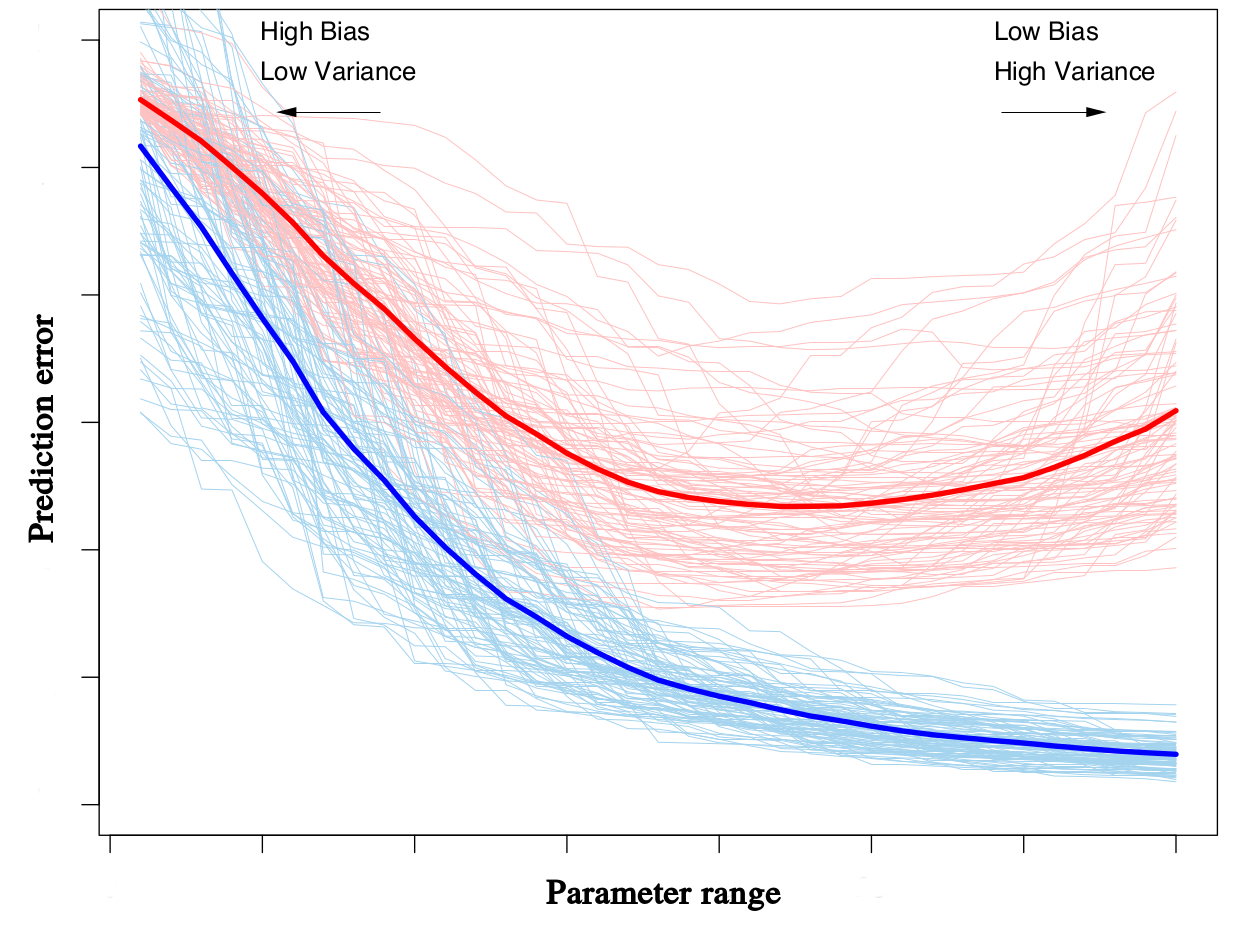
\includegraphics[width=0.7\columnwidth]{./images/regression/bias-variance_tradeoff.png}
	\caption{\label{fig:bias-variance_tradeoff} Typical behavior of prediction error for testing (red) and training (blue) dataset as a function of a hyper-parameter \citep{hastie2009elements}. Different curves are for various datasets. The solid ones are expected errors (average of all curves). From left to right can be the direction of decreasing regularization or increasing model complexity.}
\end{figure}

The idea of underfitting and overfitting can be visualized in figure \ref{fig:bias-variance_tradeoff} as modified from \citet{hastie2009elements}. It shows the prediction errors for training and testing datasets as a function of a parameter. This parameter can be either the model complexity in an increasing order or the regularization parameter $ \lambda $ in a decreasing order. Models toward the left (low complexity model, or regression with a strong regularization) are underfitting. It does not fit well both the training and testing data. Toward the right, errors on the training set decrease, while those of the testing set decrease and then increase again. Models in the far right are overfitting. They fit well the training set but not the testing set. The desired model is the one such that the error on the testing set is the lowest. At this point, the model reaches its bias-variance trade-off: bias and variance do not necessarily reach their minima, but a compromise ensures the minimal error on testing data.

The idea of bias-variance trade-off can be further visualized schematically as in figure \ref{fig:bias-variance} \citep{hastie2009elements}. The blue-shaded region shows the irreducible error $ \sigma_{\n}^2 $ (due to random noise) of the training set, where the truth is at the center and all realizations are within. To fit the model, the non-regularized model space (red curve) contains all possible models, while the magenta one shows the restricted space of regularized models. Model variances are depicted as yellow curves centered at the so-called ``closest fit''. The model bias is the distance of the closest fit and the truth, which can only be reduced as increasing the model complexity or adding more features. Regularized models add estimation bias on top of the model bias but reduce the variance. The benefit of the trade-off is only when the variance is reduced more than the squared estimation bias.

\begin{figure}
\centering
	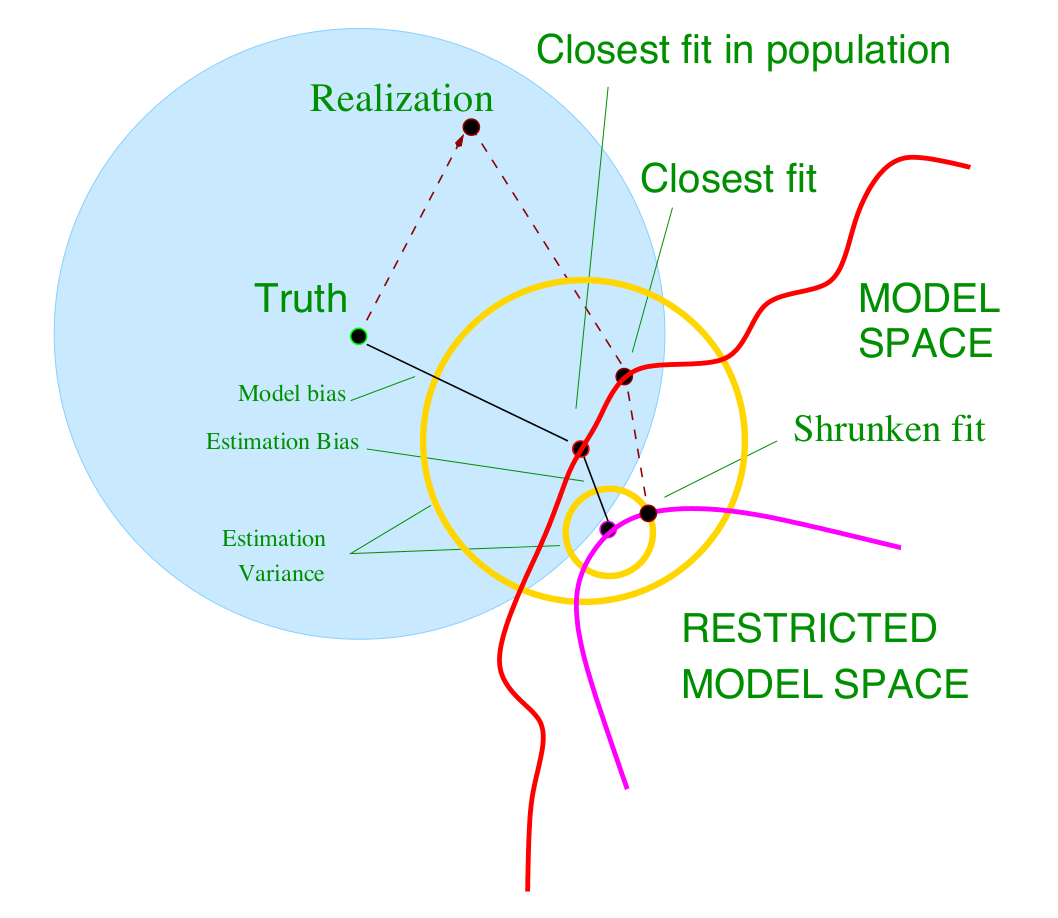
\includegraphics[width=0.6\columnwidth]{./images/regression/bias-variance.png}
	\caption{\label{fig:bias-variance} Schematic view of the behavior of bias and variance \citep{hastie2009elements}. The blue-shaded, centered at the truth, is the realization space, where maximum distance is the irreducible error. All possible models are bounded by the red/magenta model space curves. Bias is shown by the black lines as the distance to the truth. Best models are shown as black dots, and circled by model variances. }
\end{figure}

The bias-variance trade-off is essentially estimated from the training data. If this set is large enough, it can be virtually divided into training, cross-validation and testing sets. A general advice for the size of these three sets is $ 50 \% $, $ 25 \% $ and $ 25 \% $ respectively \citep{hastie2009elements}. However, learned models are usually improved when using more data. Cross-validation is another idea to find the trade-off while keeping the whole training data for learning the model. 

\subsection{Cross-validation}
In many cases, the training data is limited. Setting aside $ 50 \% $ the data to quantify the model might lose all the benefits from regularization and nonlinearity compared to OLS. Cross validation (CV) is commonly used to select the model and optimize parameters using all given data. 

The most popular CV technique is \textit{k-fold} CV. The dataset is randomly split into $ K $ subsets of approximately equal size. For each $ K $-th subset to estimate the prediction error, the model is trained on the remaining $ K-1 $ subsets. This procedure is repeated $ K $ times for all the subset, and the model error for the current setting is the average of its $ K $ estimates. A summary of k-fold CV is presented in algorithm \ref{algo_kfold}. $ K $ is at most the number of training samples (\textit{leave one out cross validation}). When $ K $ is high, the selected model tends to have lower bias but higher variance, since many training samples are similar. A much heavier computation is also required, since the training/predicting is repeated $ K $ times. The popular choice of $ K $ is from 5 to 10 \citep{breiman1992submodel, kohavi1995study}. 

\begin{algorithm}[t]
\caption{K-fold cross-validation for set of L parameters $ \gamma_1, \gamma_2, ..., \gamma_L $} \label{algo_kfold}
\begin{algorithmic}[1]
	\State Divide the training samples into k folds randomly
	\For {$ i = 1, 2, ..., L$}
		\For {$ j = 1,2,... K $}
			\State Train the model with $ \gamma_i $ using all data set except the $ j^{th} $
			\State Estimate prediction error $ \epsilon(i,j) $ of the model on the $ j^{th} $ set
		\EndFor
	\EndFor
	\State Estimate averaged error $ \epsilon(i) = \frac{1}{K}\sum\limits_{j=1}^{K}\epsilon(i,j)$
	\State Return optimal parameter $ \gamma_m $ where $ \epsilon(m) = min \{\epsilon(i)\}$.
\end{algorithmic}
\end{algorithm}

\section{Regression models for reconstruction of isotropic turbulence}
We now apply regression models to reconstruct HR velocity fields from LR measurements. The data from DNS isotropic turbulence discussed in section \ref{sec:data_isotropic} is used. Streamwise velocities from $ 37 $ data cubes of fully resolved data $ 96^3 $ are used as the reference. In each data cube, only the streamwise velocity component is considered. The training examples are the HR fields (in spanwise-vertical directions) and equivalent LR ones subsampled by a factor of $ \sqrt{\dimsh/\dimsl} = 3 $ in both vertical and spanwise directions. This ratio is equivalent to an energy loss of $ \Delta \kappa_s = 1.03 \% $ (see table \ref{tab:energyloss_isotropic}). In streamwise direction, the training planes are selected every 4 snapshots, corresponding to an energy loss of $ 1.23 \% $. This configuration is chosen to mimic other problems investigated later in chapters \ref{chap_NLM} and \ref{chap_BayesianFusion}. 

Regression models are learned from $ 37 \times 24 $ pairs of LR ($ \dimsl = 32 \times 32 $) and corresponding HR ($\dimsh = 96 \times 96 $) fields. The learned models are then used to reconstruct all $ 37 \times 96 $ HR fields from $ 37 \times 96 $ measured LR planes. These results are presented latter in chapter \ref{chap_comparisons} when comparing various methods. Following sections only discuss the optimization of model parameters.

\subsection{Regularization parameter and shrinkage effect}
Ordinary least squares model inverses directly $ \Y^{\mytrans}\Y $, which is usually ill-conditioned, leading to high variance models. A slight change of input variables can lead to very different predictions. Regularization is introduced to reduce this effect by imposing different penalty terms on regression coefficients. RR seeks a model with small sum-of-square coefficients, LASSO imposes a penalty of their absolute values (see section \ref{sec:regularized_linear_regression}). 

\begin{figure}
\centering
	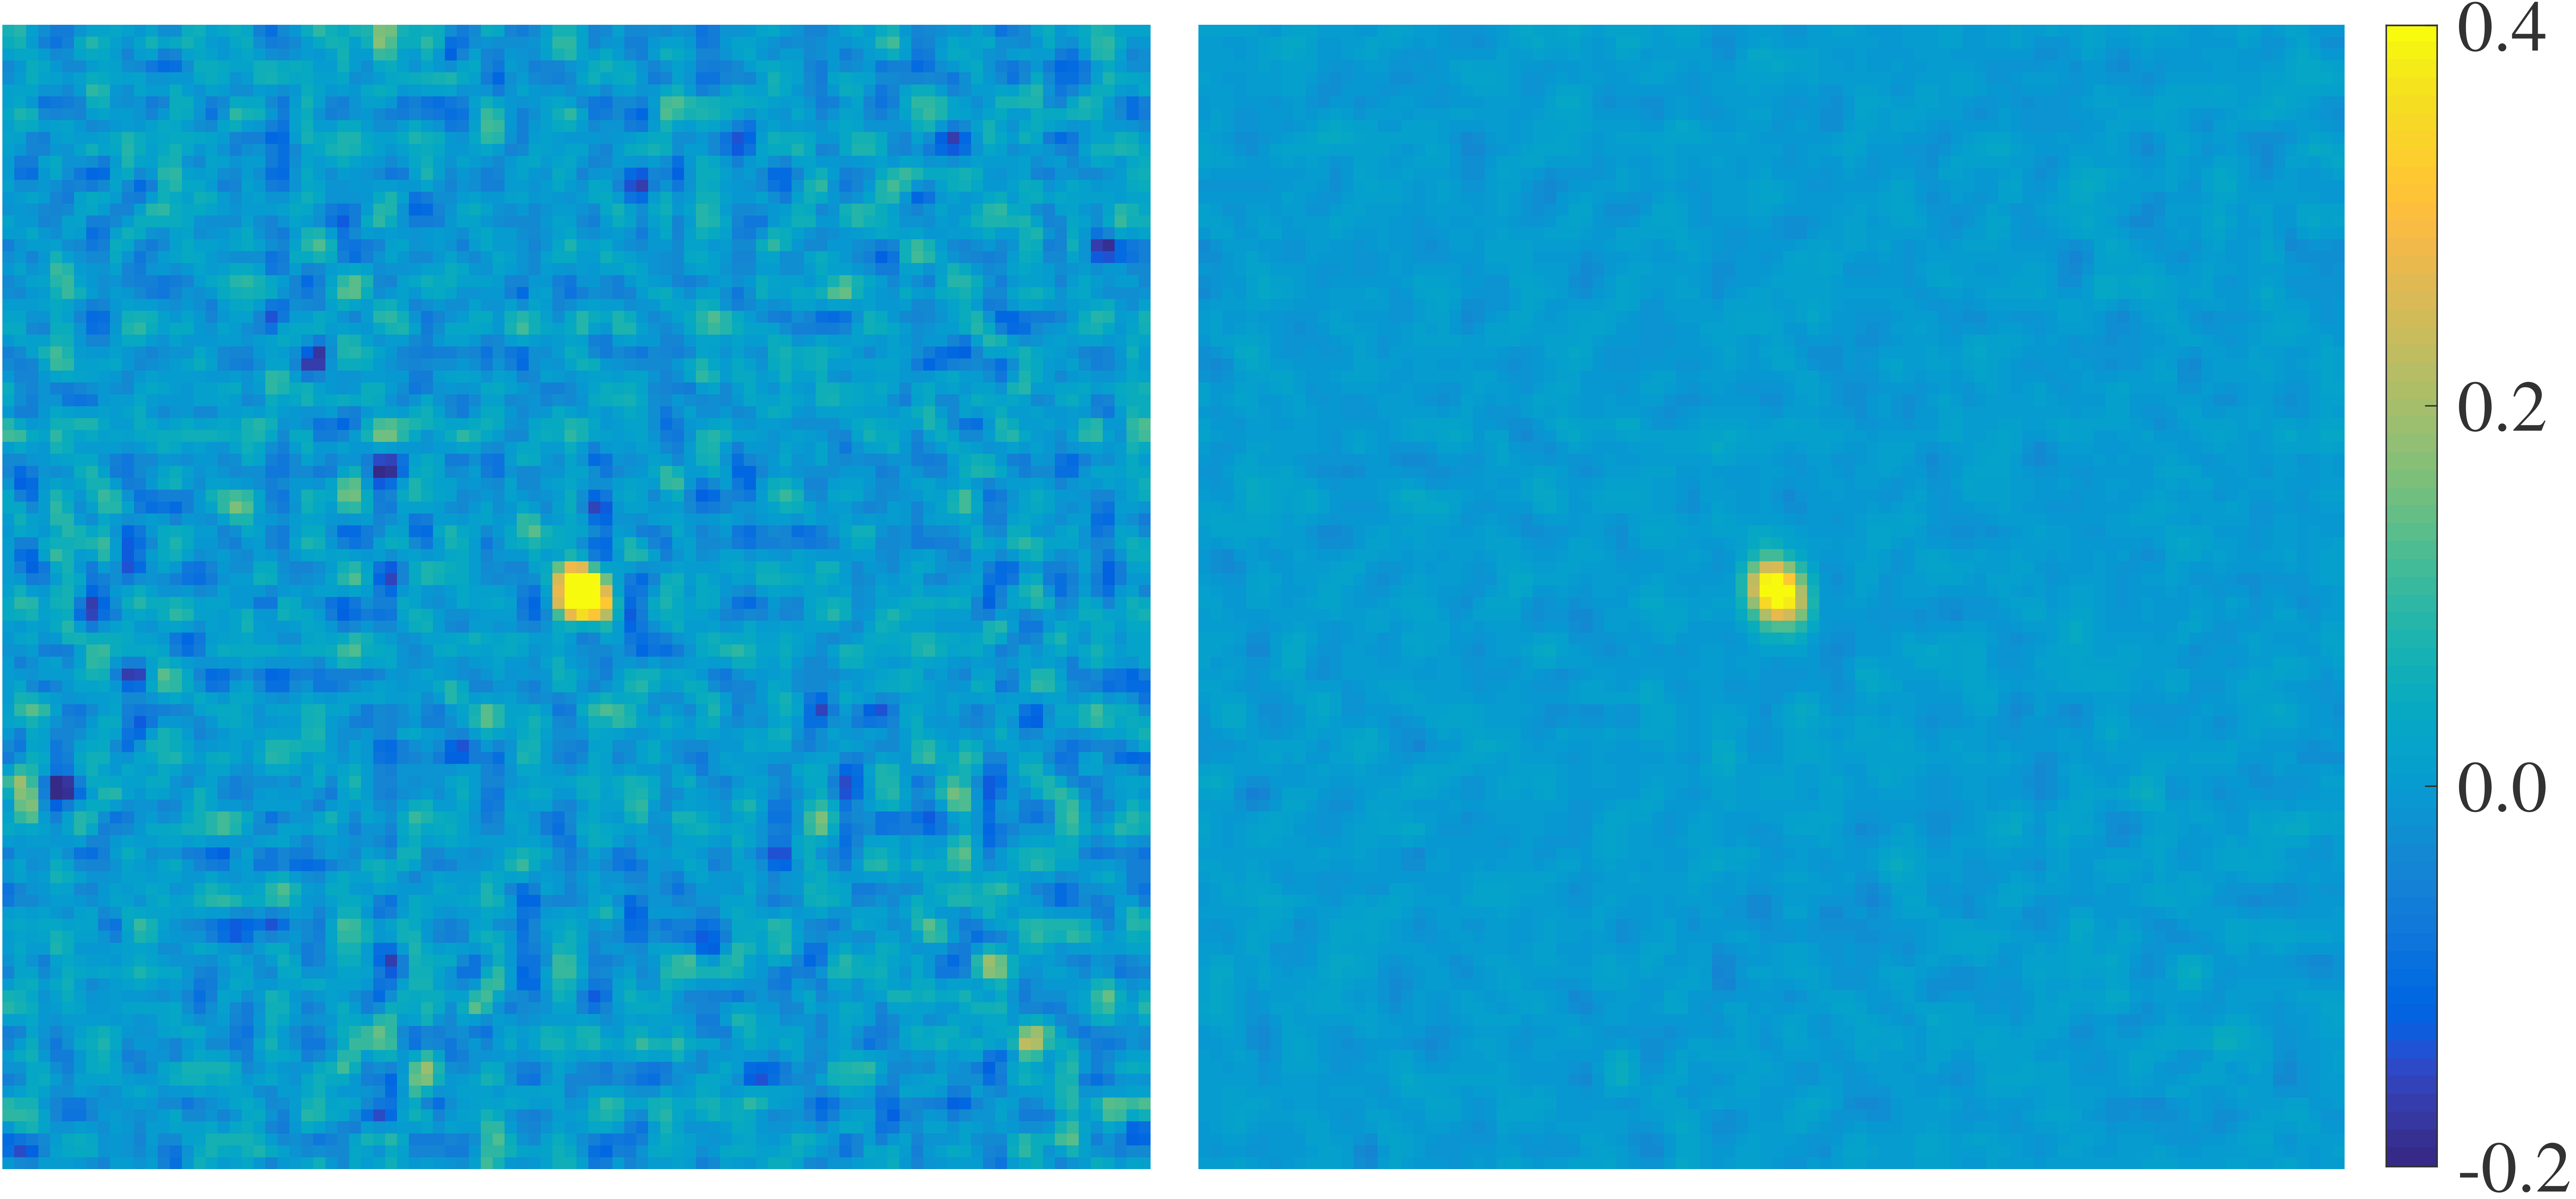
\includegraphics[width=0.8\columnwidth]{./images/regression/RR_LSE_coefficients.png}
	\caption{\label{fig:RR_LSE_coefficients} Shrinkage effect: coefficients of OLS (left) vs RR (right) models correspond to an input LR measurement at the center of the field. The coefficients, which are rearranged in a 2D field of the size $ 96 \times 96 $, can be interpreted as the contributions of this input to the reconstruction of all other high-resolution points. The higher the coefficient, the stronger the impact.}
\end{figure}

Figure \ref{fig:RR_LSE_coefficients} shows the weight of the input variable at the center of the field in reconstructing all other HR points by OLS and RR. These are the coefficients $ \mybold{b}_j \mydef [b_{j1}, b_{j2}, ..., b_{j\dimsh}]^{\mytrans}$ computed in equation \ref{eq:LSE5} for OLS or equation \ref{eq:RR2} for RR. Recall that $ \B $ is of size $ \dimsl \times \dimsh $. The figures are $ \mybold{b}_j$ of OLS and RR models, where index $ j $ corresponds to the central point. $ \mybold{b}_j $ is then rearranged to recover the 2D shape of size $ \sqrt{\dimsh} \times \sqrt{\dimsh} $ of the 2D velocity fields. In both plots, the weights remain significant in a neighborhood of several pixels. The coefficients drop very quickly when moving away from the center. This is due to the rapid decay of correlation between the central point and its neighbors. The difference between the two methods is that OLS (using direct inversion) gives large coefficients almost everywhere whereas RR shrinks the contributions of irrelevant points to small values.

\begin{figure}[t]
\centering
	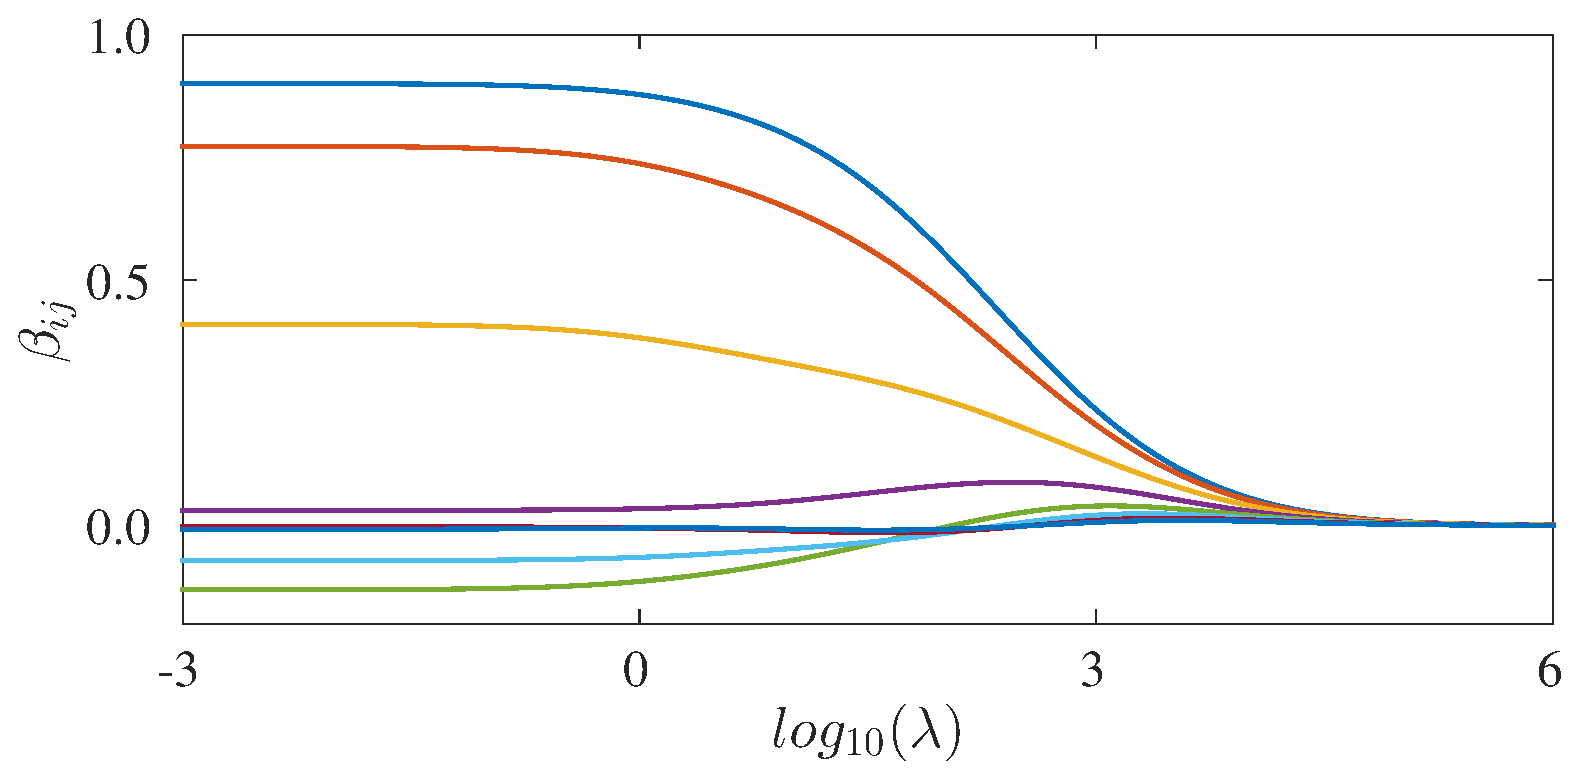
\includegraphics[width=0.8\columnwidth]{./images/regression/RR_coeffs_lambda.eps}
	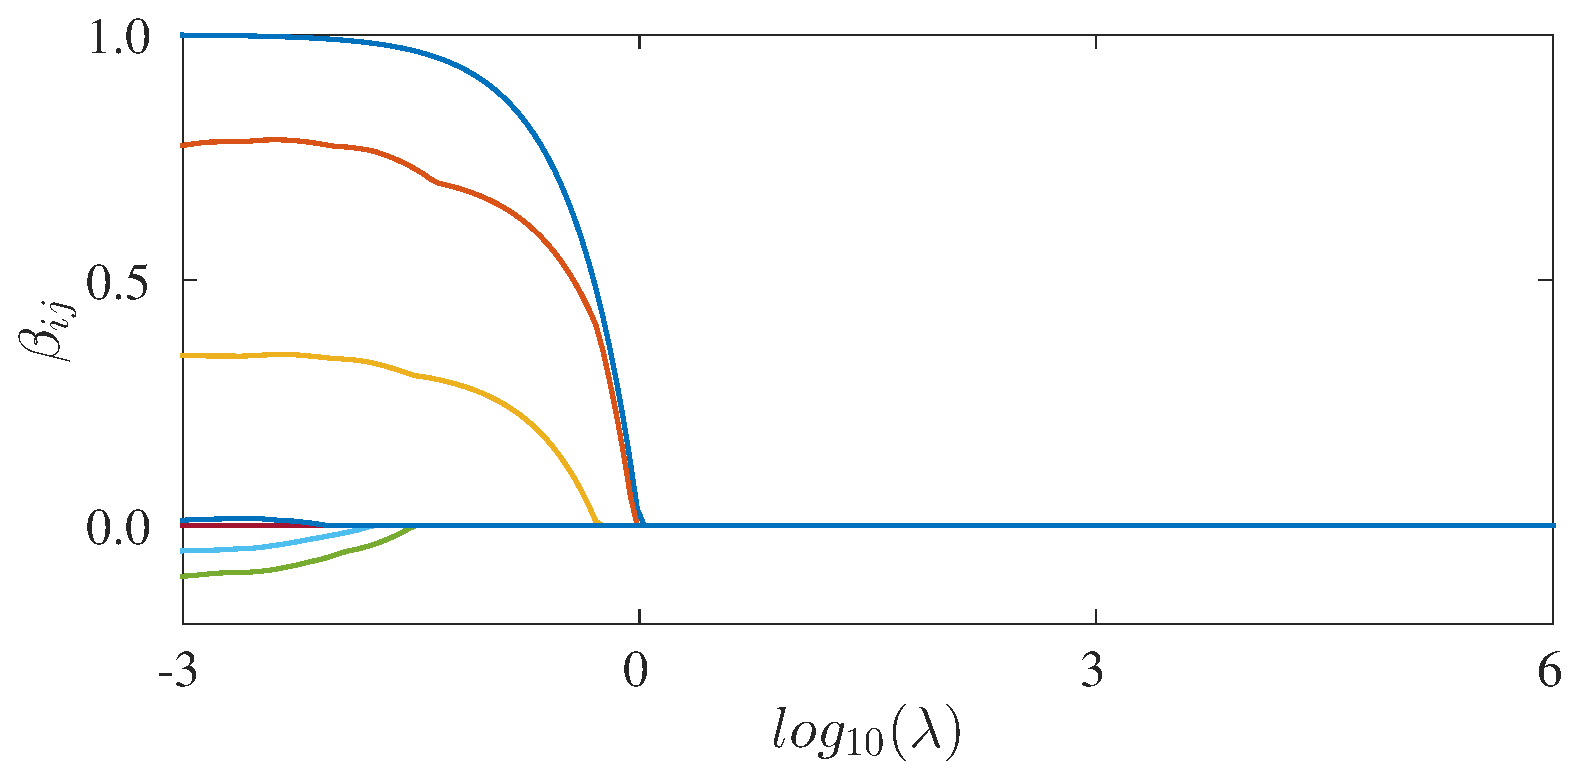
\includegraphics[width=0.8\columnwidth]{./images/regression/Lasso_coeffs_lambda.eps}
	\caption{\label{fig:coeffs_lambda} Shrinkage effects of L2 (top) and L1 (bottom) penalty: coefficients corresponding to eight high-resolution outputs (in eight different colors) as functions of regularization parameters $ \lambda $. Higher $ \lambda $ shrink the coefficients toward zeros differently depending on the penalty terms.}
\end{figure}

The different shrinkage behaviors of RR and LASSO are visualized in figure \ref{fig:coeffs_lambda}. This figure shows the eight different coefficients corresponding to eight HR outputs as a function of the regularization parameter presented in equation \ref{eq:regularized_linear_regression1}. It confirms the effect of the penalty term, which shrinks coefficients associated with irrelevant inputs to zeros. RR coefficients do not reach exact zeros even for extremely high $ \lambda $, while LASSO rapidly shrinks some coefficients to exact zeros.

\subsection{Optimizing regularization parameters and model complexity via ten-fold cross-validation}	

All regression models (except OLS) are parametric, i.e. at least one hyper-parameter controls the construction of the model and its performances. With RR, LASSO or KRR, the regularization parameter $ \lambda $ controls the balance between data misfit and regularization term. KRR model is also a function of the kernel parameter, which is the standard deviation of the distribution when using RBF kernel, or the polynomial order. All hyper-parameters are chosen from the training samples using ten-fold CV (see algorithm \ref{algo_kfold}). The plot of the error as a function of model parameters is called the ``validation curve'', from which the best model or parameter is selected.

Another important test is to see whether the training dataset is sufficient or not. This is examined via the so-called ``learning curve''. To estimate this curve, a small subset of data is drawn out randomly from the training set. This set is retained to estimate the error at the last step. For the remaining data, models are optimized using different portions. Trained models are assessed by computing prediction errors on the testing data. The curve of errors as a function of different data size, the ``learning curve'', will tell whether the current training data is sufficiently large to guarantee an accurate learning.

\begin{figure}
\centering
	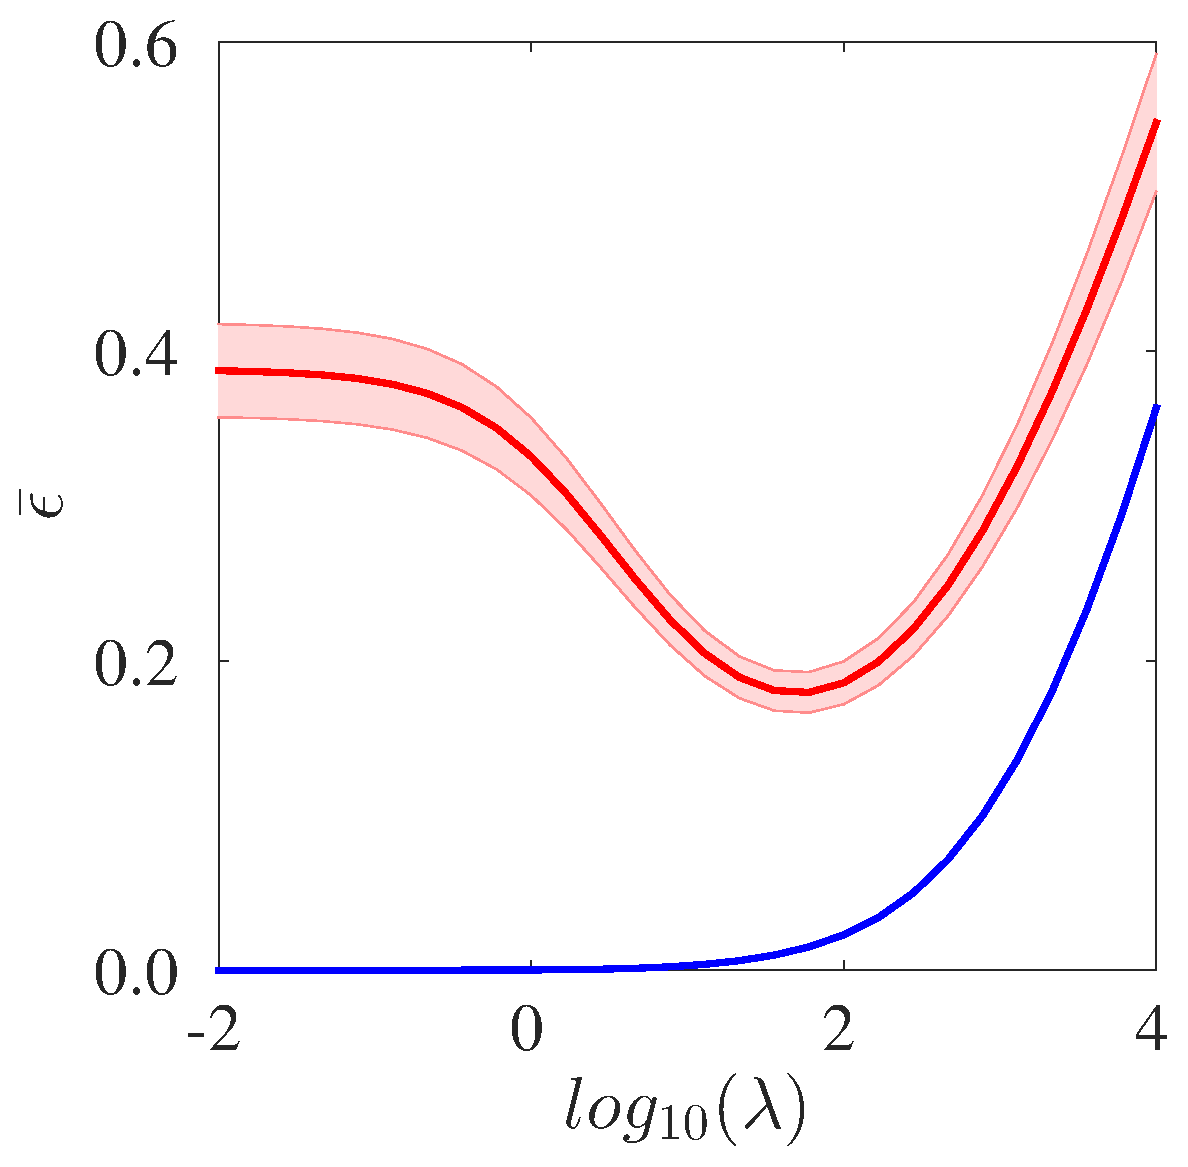
\includegraphics[height=6.75cm]{./images/regression/RR_validationcurve.eps}
	\hspace{0.3cm}
	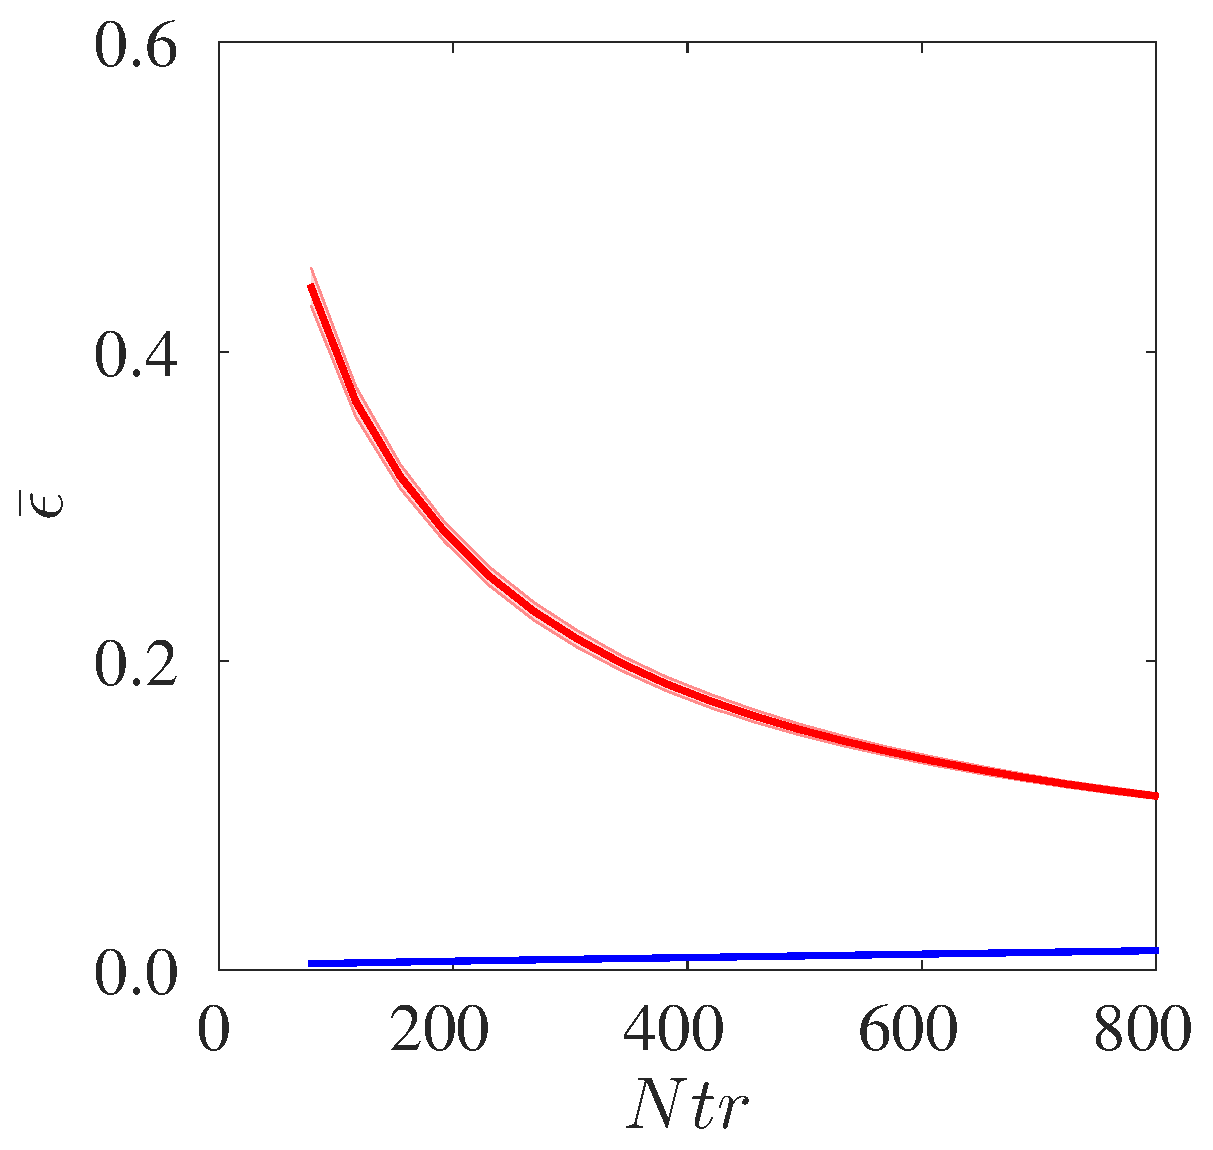
\includegraphics[height=6.75cm]{./images/regression/RR_learningcurve.eps}	
	\caption{\label{fig:RR_validationcurve} RR validation curve: errors as functions of regularization parameter $ \lambda $ (left), and learning curve: errors as functions of training data size (right). Red curves are for the prediction, while blue ones are for the training data}
\end{figure}
\begin{figure}
	\centering
	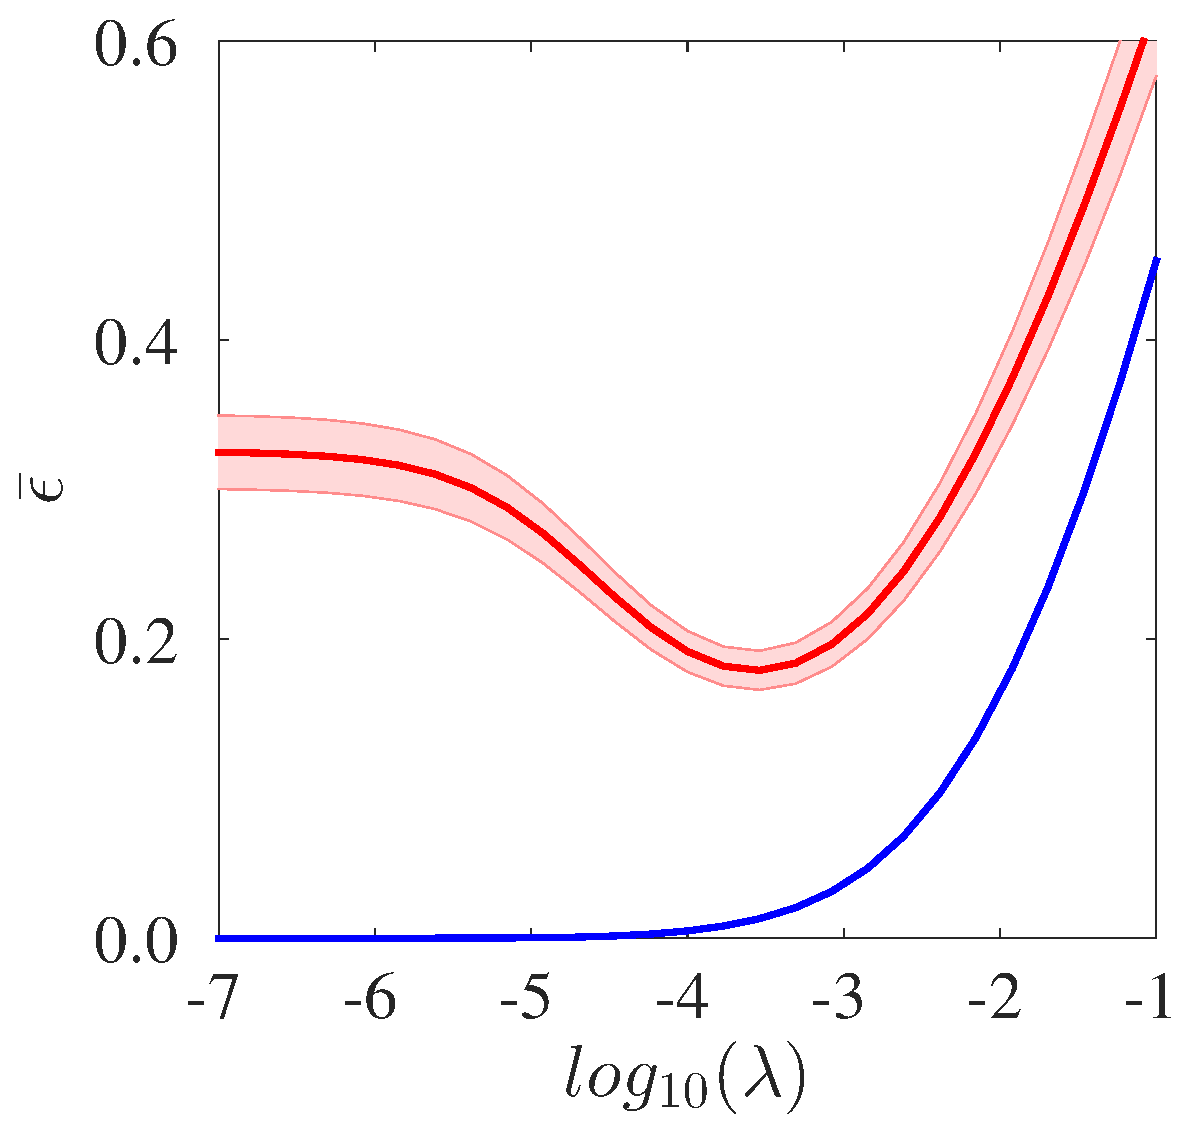
\includegraphics[height=6.75cm]{./images/regression/KRR_validationcurve_lambda.eps}
	\hspace{0.3cm}
	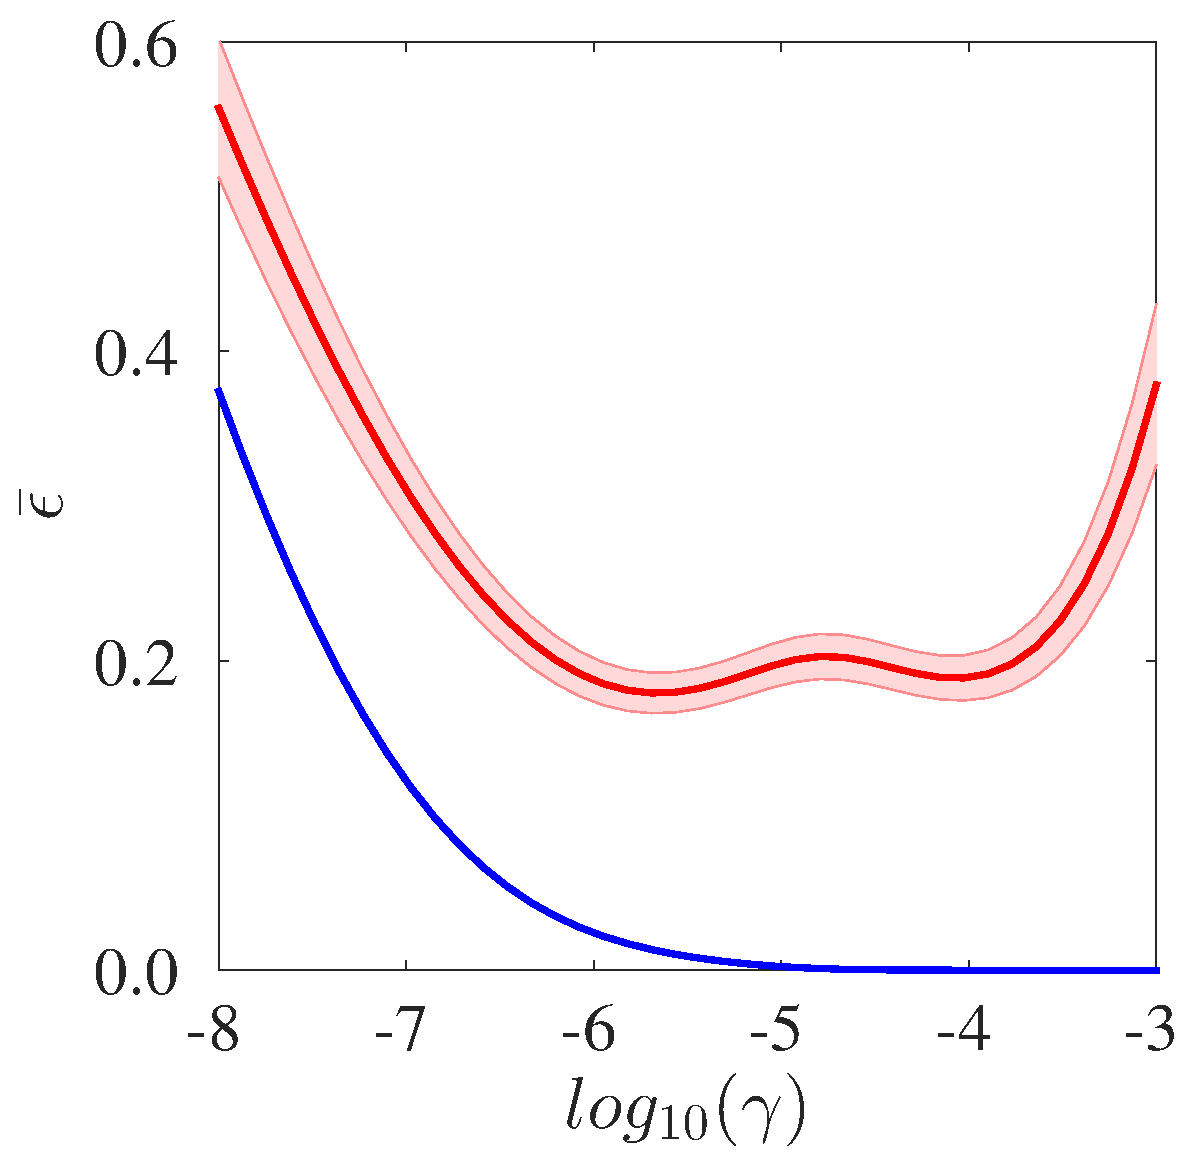
\includegraphics[height=6.75cm]{./images/regression/KRR_validationcurve_gamma.eps}	
	\caption{\label{fig:KRR_validationcurve} KRR validation curve (RBF kernel), with parameters are kernel parameter $ \gamma $ and regulartization parameter $ \lambda $. Red curves are for the prediction, while blue ones are for the training data}
\end{figure}

To plot validation and learning curves, the average normalized root mean square error (NRMSE) $ \bar{\epsilon} $ is used as the prediction error. $ \bar{\epsilon} $ represents an overall measure of the reconstruction accuracy. NRMSE is estimated between the reconstructed ($ \hat{\z}_t $) and reference ($ \z_t $) fields
\begin{equation}
\bar{\epsilon} = \left(\frac{ \sum\limits_{t} \sum\limits_{j\in \varmathbb{J}}(\hat{\mybold{z}}_{t,j}-\mybold{z}_{t,j})^2}{\sum\limits_{t} \sum\limits_{j\in \varmathbb{J}}\mybold{z}_{t,j}^2}\right)^{1/2}
\label{eq:NRMSE}
\end{equation} 
$ \varmathbb{J} $ is the considered set of points used to estimate the error. In the present case of isotropic turbulence, $ \varmathbb{J} $ contains all points in each plane.

Figure \ref{fig:RR_validationcurve} shows the validation and learning curve of RR model on the training set (blue) and validation set (red). The solid lines are the means, while a band of colors show the standard deviations of ten estimates of $ \bar{\epsilon} $ from ten folds. The validation curve (left) shows the model behavior for different $ \lambda $. For the training set, the model fits accurately the data when no or small regularization is imposed. This effect of overfitting is shown on the validation set, where higher errors are obtained. The model has also high variance, i.e. prediction errors vary strongly from one set to the other. The optimal value of $ \lambda \approx 100 $ is reached where the validation error is minimum. When a very strong regularization is imposed, errors on both training and validation sets increase, since all coefficients are shrunk toward zero. Errors will grow till their maximum value, which is the variance of the HR data. The learning curve (right) shows the effect of the training data size on the performance of the model (with optimal $ \lambda $). The figure shows that with larger training data, the prediction error on the validation set decrease sharply while this error on the training set gradually increase. With a good model and sufficiently large training data, these two curves will be very close. The curves also suggest that a larger dataset will lead to a better model in this case. 

KRR model parameters are optimized using the same validation curve. Different models come with different kernel parameters (recall table \ref{tab_basisfunctions}), together with the regularization parameter $ \lambda $. For RBF kernel, $ \gamma $ represents the kernel shape. Figure \ref{fig:KRR_validationcurve} shows that the optimal values of both $ \lambda $ and $ \gamma $ are both of the order of $ 10^{-5} $. For polynomial kernel, the polynomial order is to be tuned. The model with higher polynomial order will have lower bias but higher variance. An analogous procedure is used to find the optimal order of the polynomial fit, which is either 2 or 3 in general. 

\section{Concluding remarks}
In this chapter, regression models are used to reconstruct high resolution fields of an isotropic turbulence from low resolution measurements. The models seek a mapping function between low and high resolved fields. This function is learned from given training samples and used for prediction when only low-resolution measurements are available. 

Both linear and nonlinear models have been discussed. The ordinary least squares model is the simplest one and is widely used in the literature of turbulence. Since suffering from some critical limitations, notably overfitting and ill-conditioning, various regularization methods have been introduced. Both L2 and L1 penalty have been discussed. While L2 penalty reduces model variance by shrinking coefficients of irrelevant events, L1 forces them to zeros by slightly change the penalty term and offers some potential benefits. Nonlinear regression is another approach to improve OLS. Instead of assuming the underlying phenomenon is linear, it introduces nonlinearity by projecting input vectors to a fixed feature space before performing standard OLS. This nonlinearity helps in improving reconstruction accuracy, since assuming a linear relation between large and small scales of turbulence implies a big constraint on model performances. 

We have presented the procedure to optimize hyper-parameters of regression models. This step is crucial to ensure accurate predictions, since performances of all regression models (except OLS) depend on at least one parameter. The models are learned from the training data, but the performances are assessed on independent data only. Cross-validation is used to seek a compromise, the so-called bias-variance trade-off, from training data only. The dataset is virtually split into many subsets. The models are trained within some subsets, and their prediction generalized errors are estimated using the remaining sets. 

The optimal set of parameters is found using the validation curve and ten-fold cross validation technique. This curve shows the prediction errors on the validation set as a function of model parameters. It gives an idea of the optimal parameter range. Through all the tests, it is shown that the gradient of this curve near its minima is not very sharp, implying that a good estimate of these parameters can be achieved from the training data only. 

All model parameters are investigated. RR model is optimal when its regularization parameter $ \lambda $ is about $ 100 $. KRR model with RBF kernel is constructed with the optimal values of both $ \lambda $ and $ \gamma $ are of the order of $ 10^{-5} $. For polynomial KRR takes 2 or 3 as the optimal order of the kernel.
All such models will be used later in chapter \ref{chap_comparisons} to reconstruct high-resolution fields from low-resolution measurements and compared to other proposed methods.